\documentclass[12pt]{article}
\usepackage[utf8]{inputenc}
\usepackage[a4paper,margin=1in]{geometry}
\usepackage{amsmath} 
\usepackage{amssymb}
\usepackage{graphicx}
\usepackage{float}
\usepackage{tabularx} 
\usepackage{caption}
\usepackage{subcaption}
\usepackage{array}
\usepackage{listings}
\usepackage[dvipsnames]{xcolor}

\title{
    Department Of Aerospace Engineering,\\
    Indian Institute Of Technology Madras
    \begin{figure}[H]
        \centering
        
\includegraphics[width=8cm]{iitmlogo.png}
    \end{figure}
    \begin{center}
        \textbf{\\AS2101 : Introduction to Aerospace Engineering\\}
        Report 2 : Linear Regression of a Dataset\\
    \end{center}
}
\author{
    Pranit Zope\\AE20B046
}
\date{\today}

\begin{document}
\pagenumbering{gobble}
\maketitle
\newpage
\pagenumbering{arabic}
\tableofcontents 
\listoffigures
\listoftables
\newpage

\section{Theory}
    Linear Regression is basically a method using which we can find the line of best fit, in a scattered plot of a given dataset.
    The main use of this technique is to predict or to "forecast" the value of a dependant variable.\\
    \\For instance, we have a scattered plot, which doesn't have any particular fixed pattern. Using linear regression, we can obtain a line, that best fits and that can best predict the value of the dependant variable, using just the line and the independant variable.\\
    \\When there is only one dependant variable, it is called \textbf{Simple Linear Regression}.\\
    Figure \ref{fig:regression} explains what linear regression exactly is :
    \begin{figure}[!h]
        \centering
        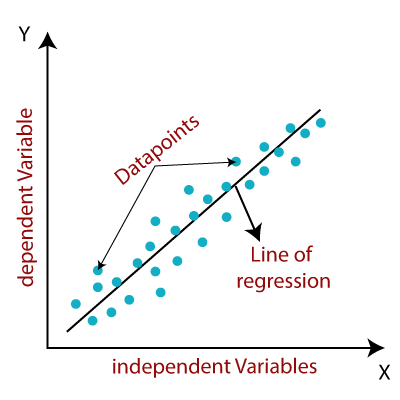
\includegraphics[width=6cm]{regression.png}
        \caption{Linear Regression of a Scattered Plot}
        \label{fig:regression}
    \end{figure}
    
\section{Procedure}
    
    \subsection{Procedure for Linear Regression}
        Let us suppose we are given a data $(x_1,y_1),(x_2,y_2),(x_3,y_3) .... (x_n,y_n)$.
        This data is a scattered, or rather a non linear plot. Our aim is to find a best fitting line $y=mx+c$ for the given dataset.
        \begin{equation}
            y=mx+c
        \end{equation}
        $m$ = slope of the line\\
        $c$ = $y$-intercept of the line\\
        Now, we will try to fit the data into the line that we just got.\\
        \begin{center}
            $y_1=mx_1+c$\\    
            $y_2=mx_2+c$\\
            $y_3=mx_3+c$\\
            $\cdot$\\
            $\cdot$\\
            $\cdot$\\
            $y_3=mx_3+c$\\
        \end{center}
        On close observation, we can see that these sets f equations can be represesnted by a matrix multiplication.
        \begin{equation}
            \begin{bmatrix}
                x_1  &  1\\
                x_2  &  1\\
                \cdot  &  \cdot\\
                \cdot  &  \cdot\\
                \cdot  &  \cdot\\
                x_n  &  1\\
            \end{bmatrix}
            \cdot
            \begin{bmatrix}
                m\\
                c
            \end{bmatrix}
            =
            \begin{bmatrix}
                y_1\\
                y_2\\
                \cdot\\
                \cdot\\
                \cdot\\
                y_n\\
            \end{bmatrix}
            \label{equ:multiplication}
        \end{equation}
    Now, here, our aim is to find out the values of $m$ and $c$, so that we can get the best fitting line.
        \begin{equation*}
            \begin{bmatrix}
                x_1  &  1\\
                x_2  &  1\\
                \cdot  &  \cdot\\
                \cdot  &  \cdot\\
                \cdot  &  \cdot\\
                x_n  &  1\\
            \end{bmatrix}
            =A  ;  
            \begin{bmatrix}
                m\\
                c
            \end{bmatrix}
            = X ;
            \begin{bmatrix}
                y_1\\
                y_2\\
                \cdot\\
                \cdot\\
                \cdot\\
                y_n\\
            \end{bmatrix}
            = B;
            \label{equ:matrix}
        \end{equation*}
        Thus we can say that in this case, $AX=B$.
        Now we can simply 
        \begin{center}
            $AX=B$\\
            $X=A^{-1}B$
        \end{center}
        But here, the problem is that $A$ is a $N \times 2$ matrix and finding its inverse is a tedious task. So we multiply by the transpose of $A$ and then compute the inverse so that the matrix will be a $2 \times 2$ matrix and Gauss-Jordan Elimination can be used.
        \begin{center}
            $AX=B$\\
            $A^TAX=A^TB$
        \end{center}
        \begin{equation}
            X = (A^TA)^{-1}A^TB
        \end{equation}
            
     
        
        Now that we have the final expression for $X$, that is
        $
        \begin{bmatrix}
            m\\
            c
        \end{bmatrix}
        $
        we can calculate it and achieve our aim.
        
    \subsection{Gauss Jordan Elimination for Inverse}
        This is a technique which is used to compute inverse of a square matrix. We take our Data matrix and one identity augmented matrix and perform row/column operations to find the inverse.
        \begin{equation}
            \begin{bmatrix}
                A|I
            \end{bmatrix}
            = 
            \begin{bmatrix}
                a & b & \bigm| 1 & 0\\
                c & d & \bigm| 1 & 0
            \end{bmatrix}
        \end{equation}
        In the case of a $2 \times 2$ matrix, the equation solves to
        \begin{equation*}
            \begin{bmatrix}
                1 & 0 & \bigm| \frac{d}{ad-bc} & \frac{-b}{ad-bc}\\
                0 & 1 & \bigm| \frac{-c}{ad-bc} & \frac{a}{ad-bc}
            \end{bmatrix}
        \end{equation*}
        Which implies that 
        \begin{equation}
            A^{-1} =
            \begin{bmatrix}
                a & b\\
                c & d
            \end{bmatrix}^{-1} = 
            \begin{bmatrix}
                \frac{d}{\Delta_A} & \frac{-b}{\Delta_A}\\
                \frac{-c}{\Delta_A} & \frac{a}{\Delta_A}
            \end{bmatrix} = \frac{1}{\Delta_A}
            \begin{bmatrix}
                d & -b\\
                -c & a
            \end{bmatrix}
        \end{equation}
        Where $\Delta_A$ is the determinant of matrix $A$.
        
    \subsection{Error Calculation}
        After figuring out our $X$ matrix, we now need ti find the error. For this, at a particular $x$ value, we will simply take the square-sum of the difference in the $y$ values and the sqrt it later.
        So, for a given $x$, our error will be 
        \begin{equation*}
            e = |y_i - (mx_i + c)|
        \end{equation*}
        Now our total error will be given by
        \begin{equation}
            E = \sqrt{\sum_{i=1}^n{e_i^2}}
        \end{equation}

\newpage        

\section{Analysis of Datasets}
    \subsection{Data 1}
        \subsubsection{Data Table}
            \begin{table}[H]
                \centering
                \begin{tabular}{|c||c|c|c|}
                \hline
                \textbf{Dataset Points} & \textbf{Slope($m$)} & \textbf{Intercept($c$)} & \textbf{Error ($E$)} \\ 
                \hline
                Points 1-50  & 7.099999999999998 & -43.19999999999993 & 131.62978386368337 \\ 
                \hline
                Points 51-100 & 17.099999999999966 & -548.2000000000007 & 131.62978386368334 \\
                \hline
                Point 10-200 & 32.09999999999991 & -2180.699999999997 & 745.1696451144531 \\
                \hline
                Points 1-200 & 22.099999999999994 & -675.6999999999998 & 4216.106687454671 \\  
                \hline
                \end{tabular}
                \caption{Data Table for Dataset 1}
                \label{tab:data1}
            \end{table}
            
        \subsubsection{Plots}
            \begin{figure}[H]
                \centering
                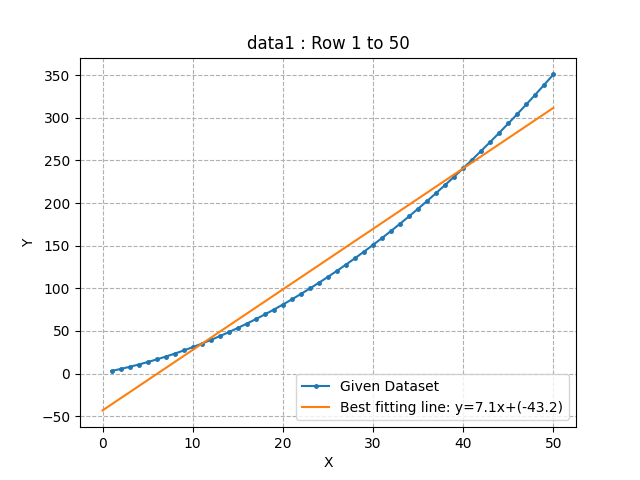
\includegraphics[width=9cm]{plot.1.1.png}
                \caption{Data 1 : Points 1-50}
                \label{fig:1.1}
            \end{figure}
            \begin{figure}[H]
                \centering
                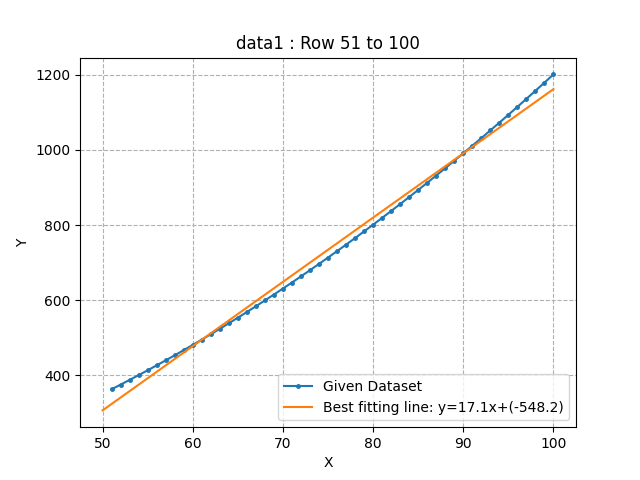
\includegraphics[width=9cm]{plot.1.2.png}
                \caption{Data 1 : Points 51-100}
                \label{fig:1.2}
            \end{figure}
            \begin{figure}[H]
                \centering
                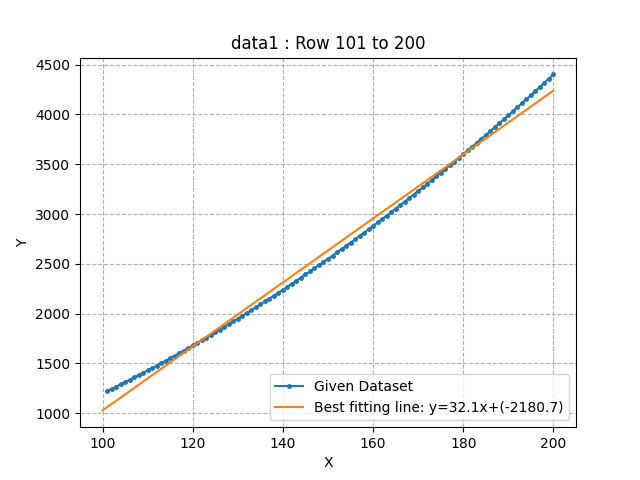
\includegraphics[width=9cm]{plot.1.3.png}
                \caption{Data 1 : Points 101-200}
                \label{fig:1.3}
            \end{figure}
            \begin{figure}[H]
                \centering
                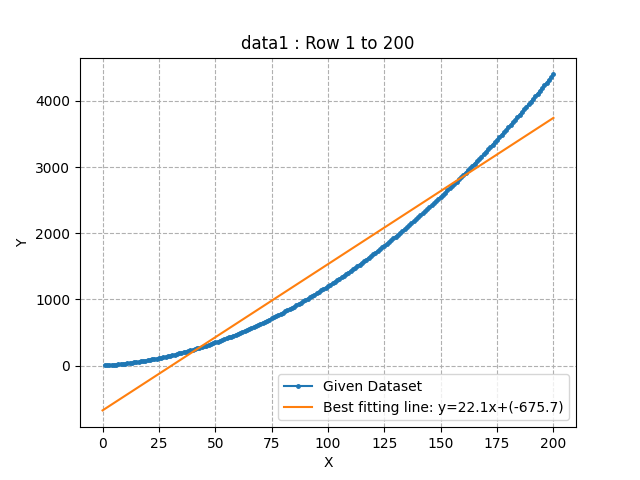
\includegraphics[width=9cm]{plot.1.4.png}
                \caption{Data 1 : Points 1-200}
                \label{fig:1.4}
            \end{figure}
            
        \subsubsection{Interpretation}
                We can say that the line is pretty much the best as it has apparently minimised the error. But if we look in the center and the end parts, the error $e=|y_i - (mx_i + c)|$ increases.\\
                Thus, we can say that there are better curves for regression, which in this case might be a quadratic function $y=ax^2+bx+c$ or an exponential function $y=a^x$.
    \newpage
                
    \subsection{Data 2}
        \subsubsection{Data Table}
            \begin{table}[H]
                \centering
                \begin{tabular}{|c||c|c|c|}
                \hline
                \textbf{Dataset Points} & \textbf{Slope($m$)} & \textbf{Intercept($c$)} & \textbf{Error ($E$)} \\ 
                \hline
                Points 1-50  & 2.01107598559424 & 1.1956343673468837 & 0.2121550871363664 \\ 
                \hline
                Points 51-100  & 2.0058037358943466 & 1.426665939976374 & 0.025965351407384034 \\
                \hline
                Points 101-200  & 2.004110508250804 & 1.6023905082547572 & 0.05222547822258797 \\
                \hline
                Points 1-200  & 2.0056244629115776 & 1.3809824773861692 & 0.9143398808678752 \\
                \hline
                \end{tabular}
                \caption{Data Table for Dataset 2}
                \label{tab:data2}
            \end{table}
            
        \subsubsection{Plots}
            \begin{figure}[H]
                \centering
                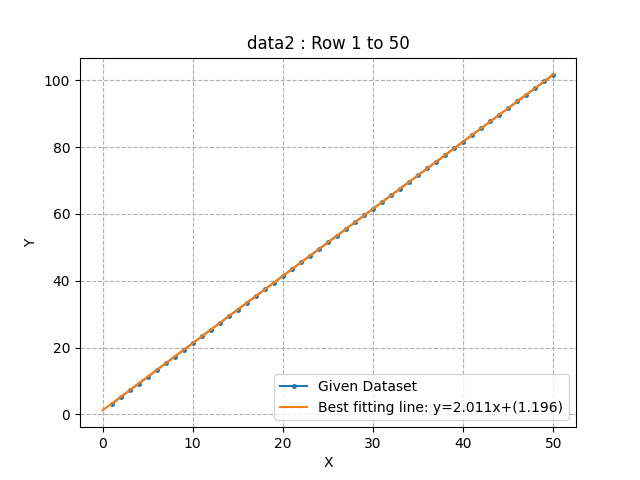
\includegraphics[width=10cm]{plot.2.1.png}
                \caption{Data 2 : Points 1-50}
                \label{fig:2.1}
            \end{figure}
            \begin{figure}[H]
                \centering
                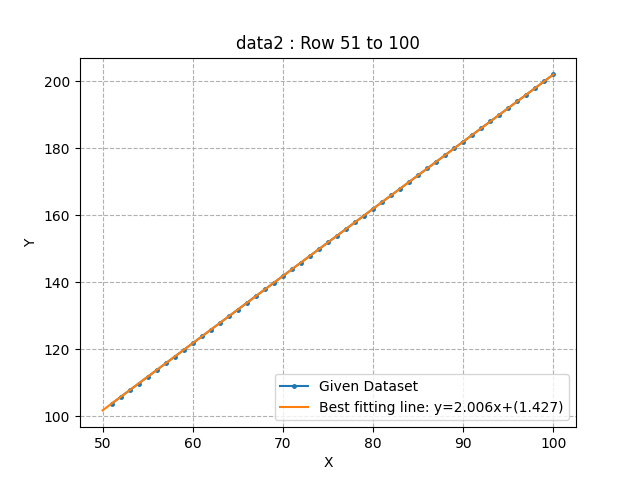
\includegraphics[width=10cm]{plot.2.2.png}
                \caption{Data 2 : Points 51-100}
                \label{fig:2.2}
            \end{figure}
            \begin{figure}[H]
                \centering
                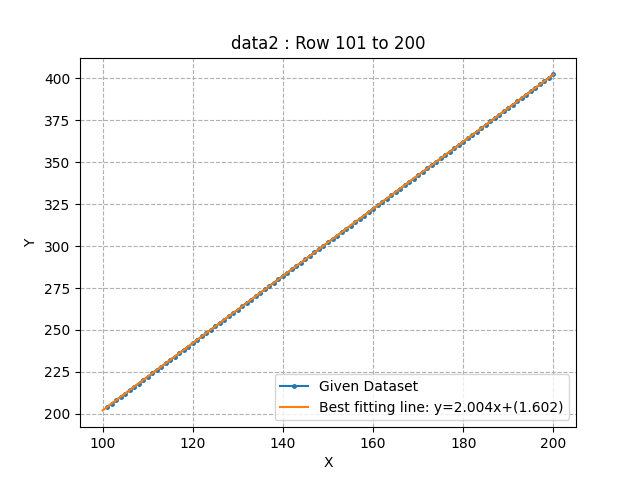
\includegraphics[width=10cm]{plot.2.3.png}
                \caption{Data 2 : Points 101-200}
                \label{fig:2.3}
            \end{figure}
            \begin{figure}[H]
                \centering
                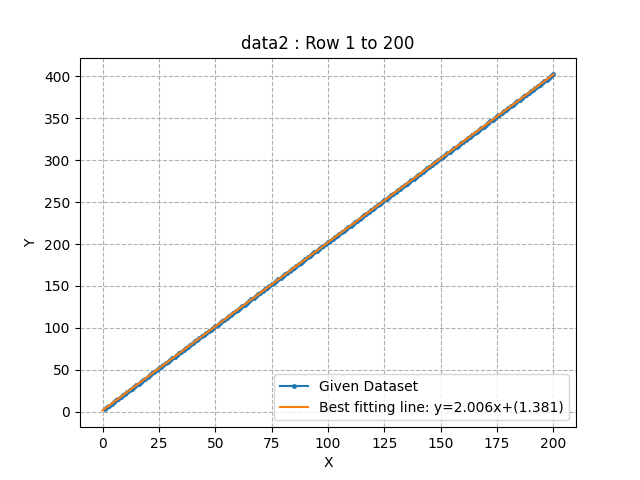
\includegraphics[width=10cm]{plot.2.4.png}
                \caption{Data 2 : Points 1-200}
                \label{fig:2.4}
            \end{figure}
            
        \subsubsection{Interpretation}
                Here we  can see that the scattered data is almost linear and the error is also very less, so we can say that linear regression is a good choice fir this dataset.
    \newpage
                
    \subsection{Data 3}
        \subsubsection{Data Table}
            \begin{table}[H]
                \centering
                \begin{tabular}{|c||c|c|c|}
                \hline
                \textbf{Dataset Points} & \textbf{Slope($m$)} & \textbf{Intercept($c$)} & \textbf{Error ($E$)} \\ 
                \hline
                 Points 1-50  & 2.0000503337334905 & 1.0036004897959856 & 0.019092074017140144 \\ 
                \hline
                Points 51-100  & 1.999962252100822 & 1.0073759663873716 & 0.02328345739436074 \\
                \hline
                Points 101-200   & 2.0000151983198364 & 1.0027986528639303 & 0.02866100570048151 \\
                \hline
                Points 1-200  & 2.0000042825320685 & 1.0044651055268332 & 0.04227031505781017 \\ [1ex] 
                \hline
                \end{tabular}
                \caption{Data Table for Dataset 3}
                \label{tab:data3}
            \end{table}
            
        \subsubsection{Plots}
            \begin{figure}[H]
                \centering
                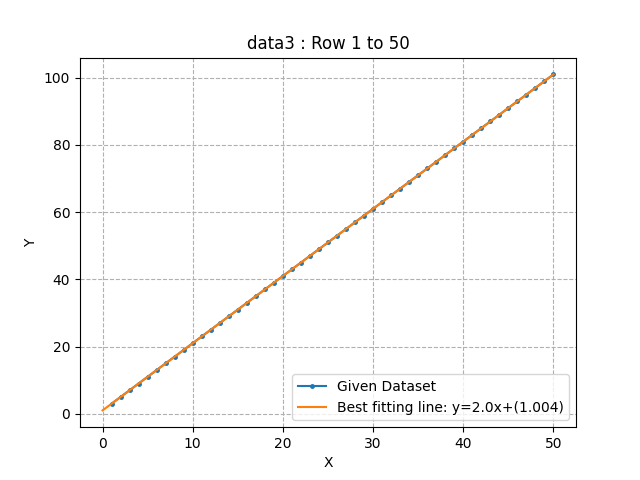
\includegraphics[width=10cm]{plot.3.1.png}
                \caption{Data 3 : Points 1-50}
                \label{fig:2.1}
            \end{figure}
            \begin{figure}[H]
                \centering
                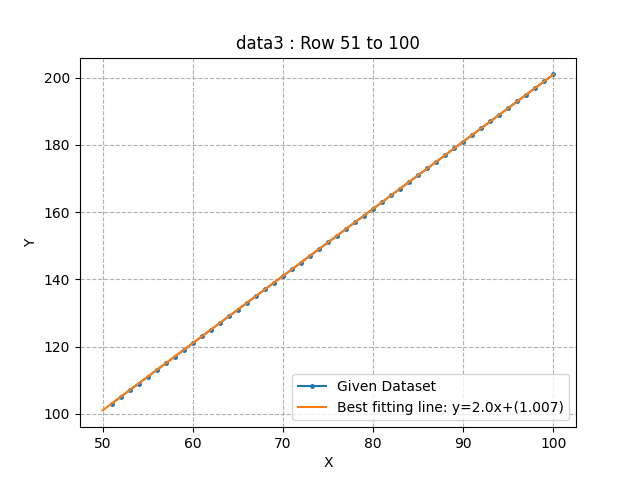
\includegraphics[width=10cm]{plot.3.2.png}
                \caption{Data 3 : Points 51-100}
                \label{fig:2.2}
            \end{figure}
            \begin{figure}[H]
                \centering
                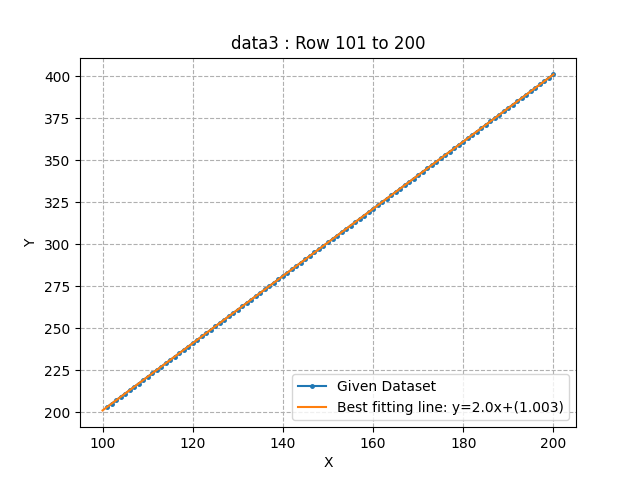
\includegraphics[width=10cm]{plot.3.3.png}
                \caption{Data 3 : Points 101-200}
                \label{fig:2.3}
            \end{figure}
            \begin{figure}[H]
                \centering
                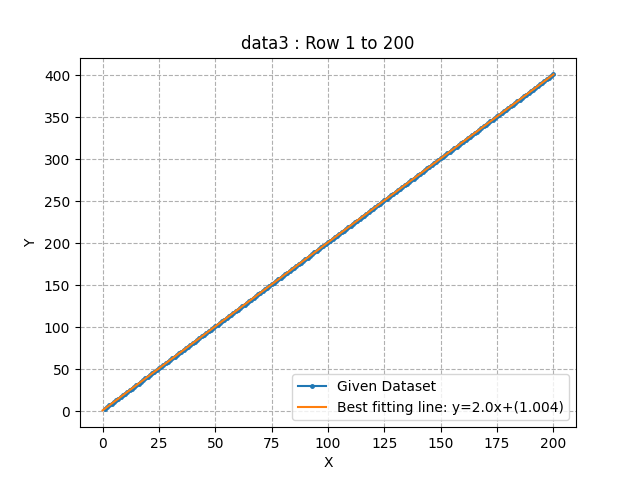
\includegraphics[width=10cm]{plot.3.4.png}
                \caption{Data 3 : Points 1-200}
                \label{fig:2.4}
            \end{figure}
            
        \subsubsection{Interpretation}
                Here we  can see that the scattered data is almost linear and the error is also very less, so we can say that linear regression is a good choice fir this dataset.                
    \newpage

\end{document}

